\section{Evaluation}\label{sec:eval}

\begin{figure*}
  \centering
  \begin{subfigure}[b]{0.24\textwidth}
    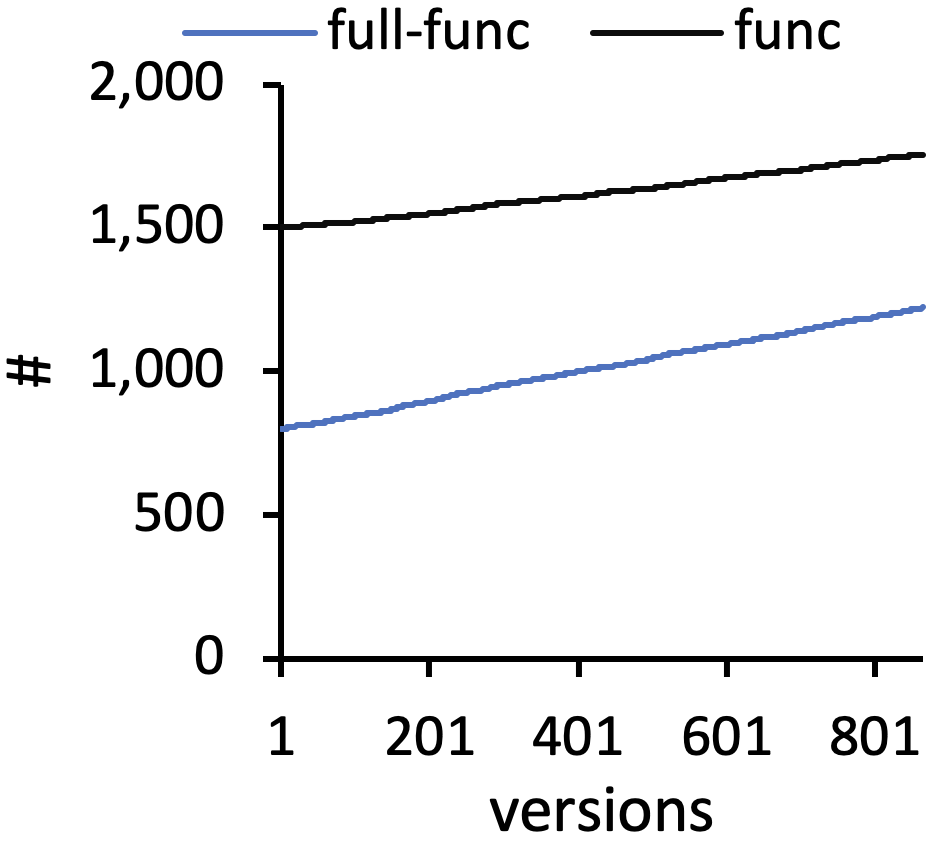
\includegraphics[width=\textwidth]{img/func}
    \caption{The number of functions.}
  \end{subfigure}
  \begin{subfigure}[b]{0.24\textwidth}
    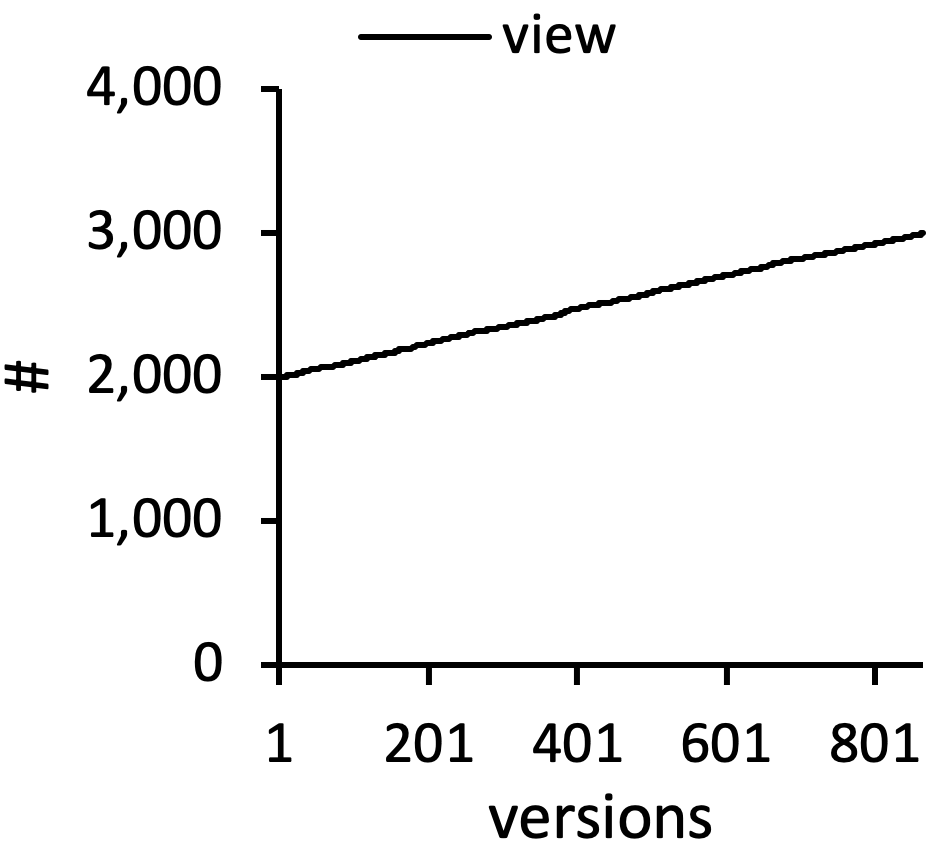
\includegraphics[width=\textwidth]{img/view}
    \caption{The number of views.}
  \end{subfigure}
  \begin{subfigure}[b]{0.24\textwidth}
    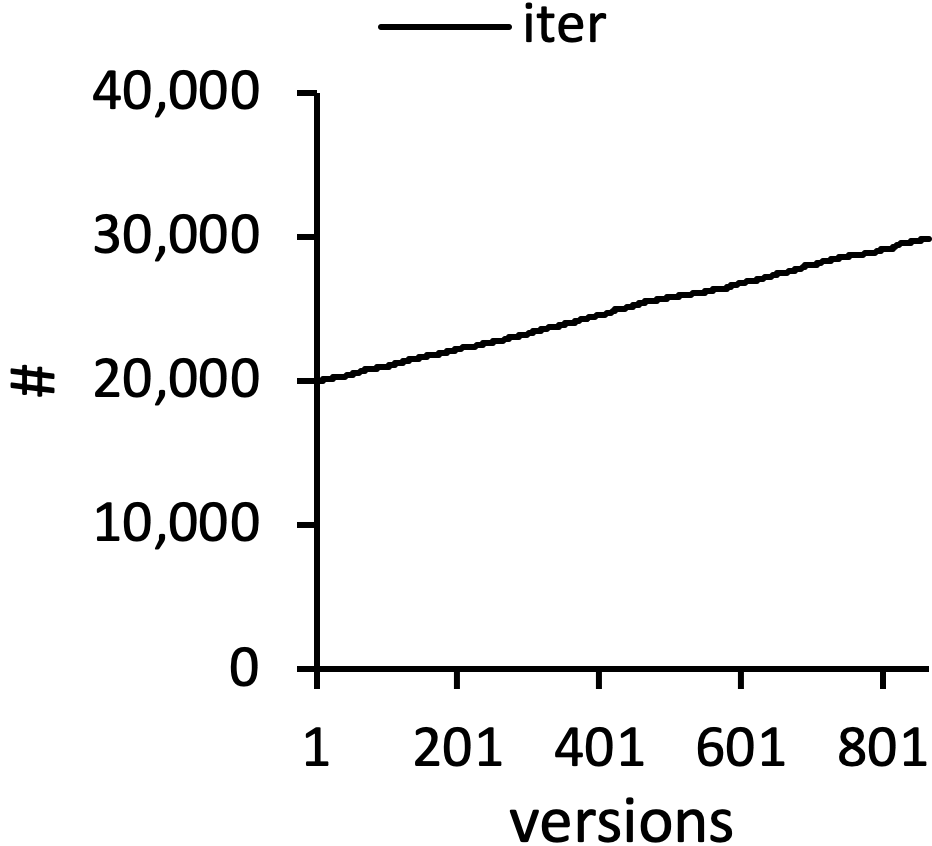
\includegraphics[width=\textwidth]{img/iter}
    \caption{The number of iterations.}
  \end{subfigure}
  \begin{subfigure}[b]{0.24\textwidth}
    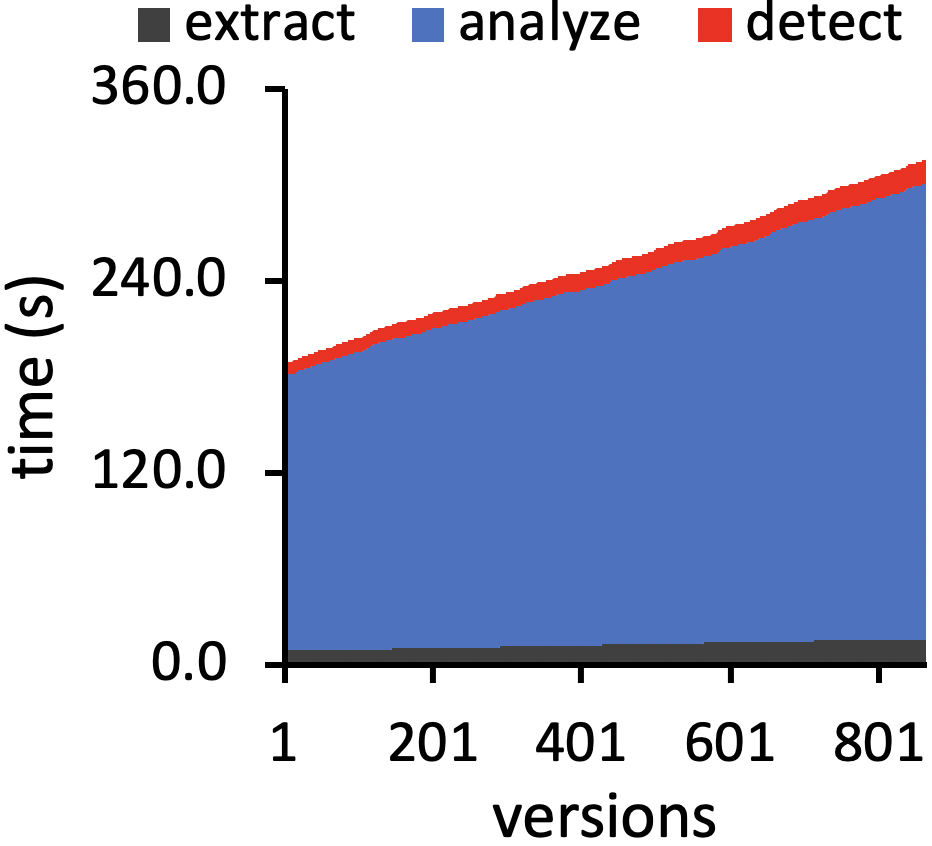
\includegraphics[width=\textwidth]{img/time}
    \caption{The analysis time.}
  \end{subfigure}
  \caption{The statistics of $\tool$ for each version of ECMAScript.}
  \label{fig:stat}
\end{figure*}

We implemented $\tool$ as an open-source tool~\footnote{The link is anonymized
because of a double-blind review process} in Scala by extending $\jiset$, a
JavaScript IR-based semantics extraction toolchain, with a worklist-based
fixpoint algorithm for type analysis.  Since $\jiset$ cannot automatically
compiles algorithm steps written in an uncommon writing style to $\ires$
instructions, our tool only reports type-related specification bugs detected in
fully compiled abstract algorithms.  For built-in libraries, we only targeted
abstract algorithms of essential built-in objects: \jscode{Array},
\jscode{Object}, \jscode{Function}, \jscode{Math}, \jscode{Proxy}, and objects
for primitive types.

To evaluate $\tool$, we answer the following research questions:
\begin{itemize}
  \item RQ1. \textbf{(Performance)} How long does $\tool$ take to perform type
    analysis for JavaScript specifications?
  \item RQ2. \textbf{(Precision)} How many type-related specification bugs
    detcted by $\tool$ are true bugs?
  \item RQ3. \textbf{(Effect of Refinement)} Does the condition-based refinement
    improve the analysis precision with endurable performance degradation?
  \item RQ4: \textbf{(Detection of New Bugs)} Does $\tool$ detect new
    specification bugs in the latest version of ECMAScript?
\end{itemize}
The draft of the next version of ECMAScript (ES12, 2021) is fixed on March 9,
2021.  Thus, we targeted all different \inred{864} versions existed in the
official ECMAScript repository~\footnote{https://github.com/tc39/ecma262} for
the recent three years from January 1, 2018 to March 9, 2021.  We performed our
experiments on five Ubuntu machines equipped with 4.2GHz Quad-Core Intel Core i7
and 32GB of RAM.


\subsection{Performance}

To evaluate the performance of $\tool$, we measured the analysis time for
\inred{864} versions of ECMAScript.  For each version, we assigned an unsigned
integer as its unique identifier in chronological order starting from 1; the
identifier of the oldest version is 1 and that of the latest version is
\inred{864}.  Figure~\ref{fig:time} depicts the analysis time of $\tool$ for
each version in chronological order.  The dark gray, blue, and red bars
represent times of specification extraction (\code{extract}), type analysis
(\code{analyze}), and bug detection (\code{detect}), respectively.  $\tool$ took
\inred{XXX.XX} seconds to analyze each version of ECMAScript on average; the
specification extraction took \inred{XX.XX} seconds (\inred{XX.XX}\%), the type
analysis took \inred{XX.XX} seconds (\inred{XX.XX}\%), and the bug detection
took \inred{XX.XX} seconds (\inred{XX.XX}\%) on average.


\subsection{Precision}

\begin{figure}
  \centering
  \begin{subfigure}[b]{0.24\textwidth}
    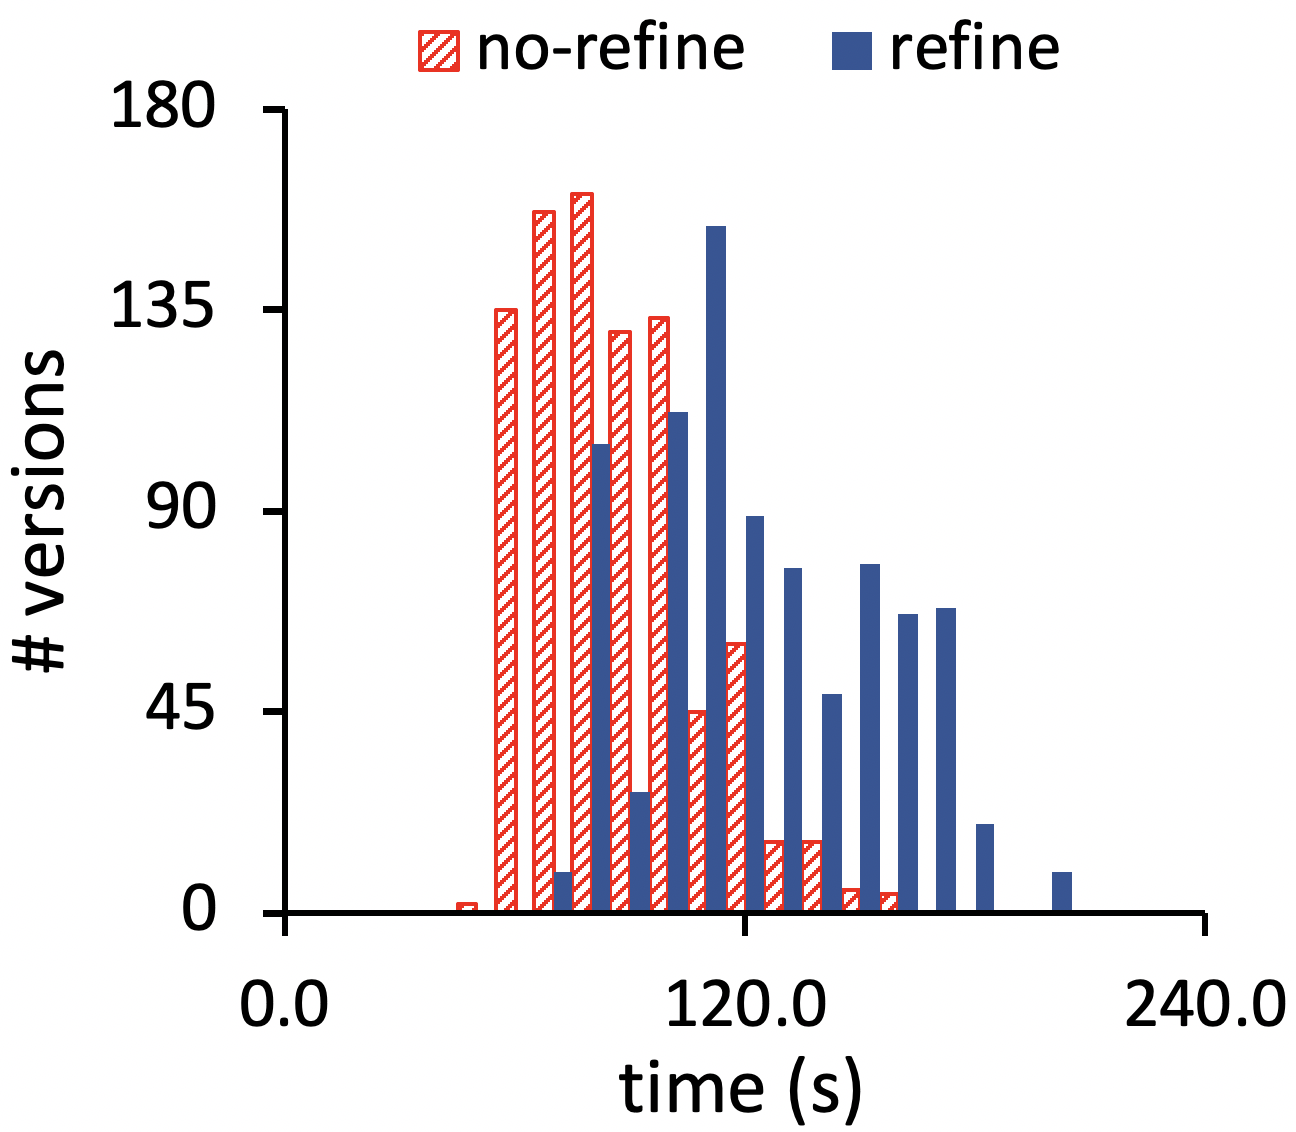
\includegraphics[width=\textwidth]{img/compare-time}
    \caption{The analysis time.}
  \end{subfigure}
  \begin{subfigure}[b]{0.24\textwidth}
    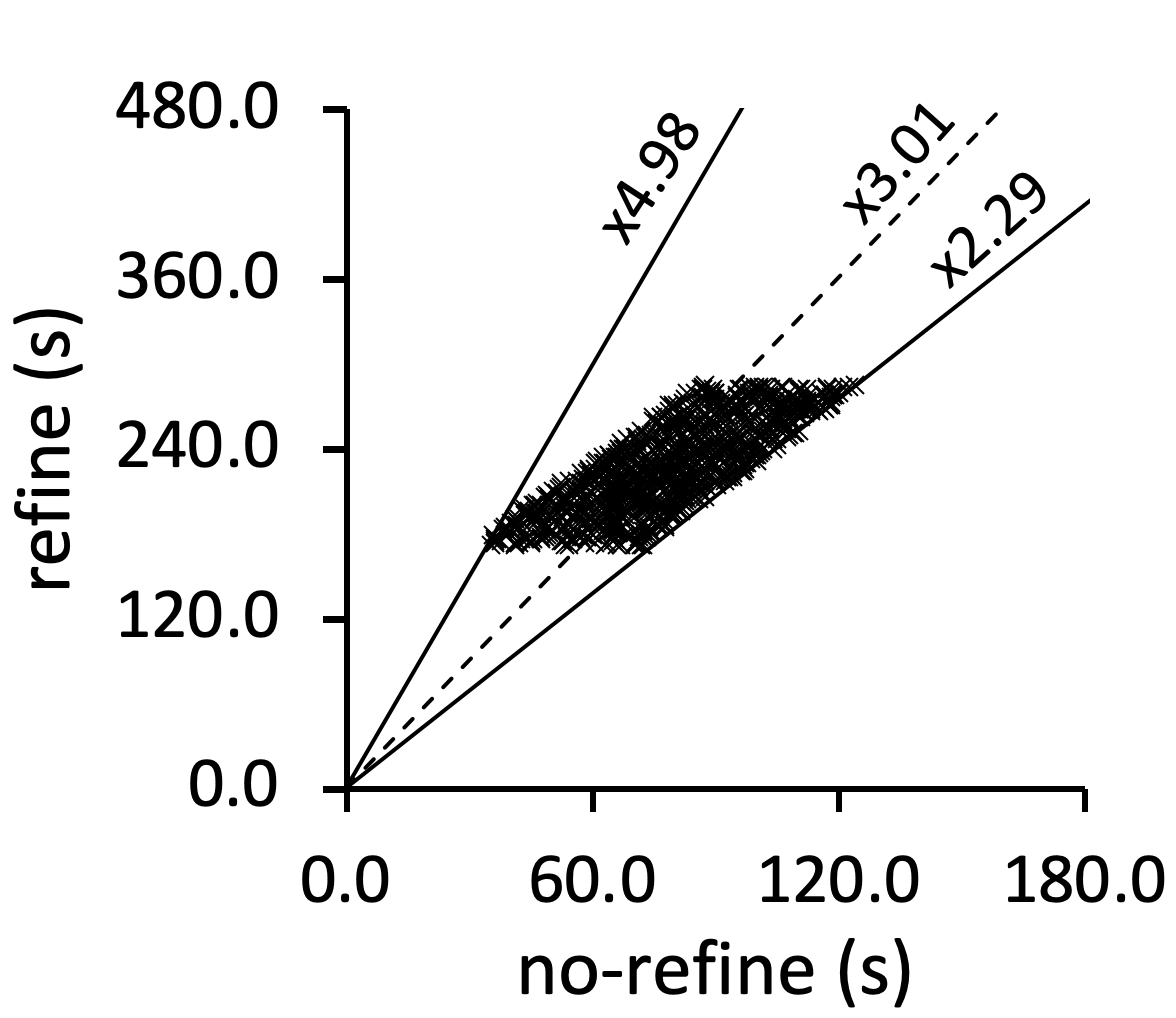
\includegraphics[width=\textwidth]{img/ratio-time}
    \caption{The ratio of analysis time.}
  \end{subfigure}
  \caption{The comparison between analysis time without and without condition-based
  refinement.}
  \label{fig:refine}
\end{figure}

\begin{table*}
  \centering
  \[
    \footnotesize
    \begin{array}{c|c?c|c?c|c?c|c}
      \multirow{2}{*}{\textbf{Checker}} &
      \multirow{2}{*}{\textbf{Bug Kind}} &
      \multicolumn{6}{c}{
        \textbf{Precision = (\# True Bugs) / (\# Total Bugs)}
      }\\\cline{3-8} &&
      \multicolumn{2}{c?}{\text{no-refine}} &
      \multicolumn{2}{c?}{\text{refine}} &
      \multicolumn{2}{c}{\Delta}\\\hline\hline

      \myrowc{2}
      {Reference}     {60 / 116 (51.7\%)} {60 / 116 (51.7\%)} {\md{12}{3}{51.7}}
      {UnknownVar}    {17 / 72 (23.6\%)}  {17 / 72 (23.6\%)}  {\md{12}{3}{51.7}}
      \myrowh
      {DuplicatedVar} {43 / 44 (97.7\%)}  {43 / 44 (97.7\%)}  {\md{12}{3}{51.7}}

      \hline

      \myrowc{2}
      {Arity}         {60 / 116 (51.7\%)} {60 / 116 (51.7\%)} {\md{12}{3}{51.7}}
      {MissParam}     {17 / 72 (23.6\%)}  {17 / 72 (23.6\%)}  {\md{12}{3}{51.7}}
      \myrowh
      {RemainArg}     {43 / 44 (97.7\%)}  {43 / 44 (97.7\%)}  {\md{12}{3}{51.7}}

      \hline

      \myrowc{1}
      {Assertion}     {60 / 116 (51.7\%)} {60 / 116 (51.7\%)} {\md{12}{3}{51.7}}
      {Assertion}     {17 / 72 (23.6\%)}  {17 / 72 (23.6\%)}  {\md{12}{3}{51.7}}

      \hline

      \myrowc{2}
      {Operand Type}  {60 / 116 (51.7\%)} {60 / 116 (51.7\%)} {\md{12}{3}{51.7}}
      {NoNumber}      {17 / 72 (23.6\%)}  {17 / 72 (23.6\%)}  {\md{12}{3}{51.7}}
      \myrowh
      {Abrupt}        {43 / 44 (97.7\%)}  {43 / 44 (97.7\%)}  {\md{12}{3}{51.7}}

      \hline\hline

      \mysrowh
      {Total}         {43 / 44 (97.7\%)}  {43 / 44 (97.7\%)}  {\md{12}{3}{51.7}}

    \end{array}
  \]
  \caption{The analysis precision of $\tool$ without and with condition-based
  refinement.}
  \label{fig:refine}
\end{table*}


  Moreover, Figure~\ref{fig:function}
represents the number of functions analyzed by $\tool$ for each version of
ECMAScript; the gray and dark gray bars denote numbers of partially and fully
compiled functions, respectively.  On average, \inred{XXXX} functions are
analyzed by $\tool$ thus 

Figure~\ref{fig:function}
Figure~\ref{fig:time}

$\tool$ consists of three steps:
specification extraction, type analysis, and bug detection, and we measured the
duration time 


For different \inred{864} versions of ECMAScript, 

We evaluated performance 


\subsection{Effectiveness of Refinement}

\todo: refinement: performance / precision


\subsection{Impact}

\todo: TTL / creater or solver / \# by kinds / new bugs
